\documentclass[a4paper,11pt]{article}

% ============================================================================
% TRABALHO FINAL - CIENCIA DE DADOS (TP2)
% UNESP - Faculdade de Ciencias - Bauru - Departamento de Computacao
%
% Tema 6 - Criminalidade urbana por regiao
% Recorte: Rio Grande do Sul, por MUNICIPIO (agrupado em mesorregioes do IBGE)
%
% ATENCAO: o enunciado sugere o "Springer Nature LaTeX Template" (Overleaf).
% Este arquivo cobre a MESMA estrutura no estilo do nextmedia.tex. Se o template
% Springer for obrigatorio, o texto abaixo migra sem alteracao - so troca o
% preambulo. Confirmar com o professor.
%
% PENDENCIAS ANTES DA ENTREGA:
%  - preencher o RA do Davi na capa (esta 000000000)
%  - revisar o texto e conferir os numeros contra a ultima execucao do notebook
% ============================================================================

\usepackage[T1]{fontenc}
\usepackage[utf8]{inputenc}
\usepackage[brazil]{babel}
\usepackage{graphicx}
\usepackage{booktabs}
\usepackage{array}
\usepackage{enumitem}
\usepackage{xcolor}
\usepackage{amsmath}
\usepackage{hyperref}
\usepackage{indentfirst}
\usepackage[top=2.2cm,bottom=2.2cm,left=2.2cm,right=2.2cm]{geometry}

\hypersetup{
    hidelinks,
    pdftitle={Criminalidade urbana no Rio Grande do Sul -- Trabalho Final de Ciencia de Dados},
    pdfauthor={Mario Masao Mukai e Davi Ferreira de Souza}
}
\urlstyle{same}

\setlength{\parindent}{1.25cm}
\setlength{\parskip}{0pt}
\graphicspath{{../figuras/}{figuras/}}

% ============================================================================
\title{\textbf{Onde e quando patrulhar?}\\[2mm]
\large Padrões espaciais e temporais da criminalidade no Rio Grande do Sul,\\
por município e mesorregião\\
\normalsize a partir dos microdados de ocorrências da SSP-RS}

\author{
Mário Masao Mukai -- RA: 241022321\\
Davi Ferreira de Souza -- RA: 000000000\\[2mm]
\small Trabalho Final -- Ciência de Dados\\
\small Universidade Estadual Paulista ``Júlio de Mesquita Filho'' (UNESP)\\
\small Faculdade de Ciências -- Bauru -- Departamento de Computação
}
\date{Bauru -- SP, \today}

\begin{document}
\maketitle

% ----------------------------------------------------------------------------
\begin{abstract}
\noindent
Uma secretaria estadual de segurança precisa distribuir um efetivo limitado
entre municípios, regiões e turnos, e costuma fazê-lo pelo volume bruto de
ocorrências, que apenas reflete o tamanho das cidades. Investigamos se há um
padrão espacial e temporal identificável na criminalidade do Rio Grande do Sul
que justifique uma alocação mais informada. Usamos os microdados de ocorrências
da SSP-RS (2022--2025, 3,1 milhões de registros) combinados com a população e as
mesorregiões do IBGE, com análise exploratória, teste qui-quadrado de
independência e teste de Kruskal-Wallis. Encontramos que o tipo de ocorrência
depende do turno de forma estatisticamente significativa, ainda que de magnitude
modesta (arrombamento de madrugada, furto de dia, roubo e lesão à noite), que o
pico é a noite em todas as sete mesorregiões, e que a taxa por habitante difere
entre regiões. Recomendamos uma escala de policiamento uniforme no pico noturno e
diferenciada por tipo de crime e região, priorizando municípios pela taxa por
habitante e tratando o litoral como caso sazonal, com a ressalva de que o dado
mede ocorrência registrada e a população de referência é a residente.

\vspace{2mm}
\noindent\textbf{Palavras-chave:} ciência de dados; segurança pública;
análise exploratória; teste de hipóteses; taxa por habitante; mesorregião.
\end{abstract}

% ============================================================================
\section{Contexto}\label{sec:contexto}
% ============================================================================
A segurança pública no Brasil é atribuição dos estados, e cabe às secretarias
estaduais distribuir um contingente policial finito por um território extenso e
heterogêneo. No Rio Grande do Sul são 497 municípios, de capitais regionais a
cidades de poucos milhares de habitantes, com dinâmicas de criminalidade
distintas. Na ausência de evidência, essa distribuição tende a seguir o volume
absoluto de ocorrências --- critério que favorece automaticamente as cidades
grandes, onde há mais pessoas e, portanto, mais registros, sem dizer nada sobre
o \emph{risco} enfrentado pelo cidadão nem sobre \emph{quando} o crime ocorre.

Padrões espaciais e temporais mudam essa conversa. Se o crime se concentra em
certos turnos, a mesma equipe rende mais quando escalada nas horas certas. Se o
risco por habitante difere entre regiões, a prioridade deixa de ser apenas a
capital. Este trabalho investiga esses padrões a partir de dados públicos e
abertos, com o objetivo de subsidiar uma decisão de alocação.

% ============================================================================
\section{Pergunta central}\label{sec:pergunta}
% ============================================================================
O Tema~6 pergunta se os tipos de ocorrência têm padrão espacial ou temporal
identificável. Ajustamos o recorte para torná-lo acionável por um órgão
estadual: \emph{no Rio Grande do Sul, os tipos de ocorrência têm padrão espacial
(por município e mesorregião) e temporal (dia da semana, horário) identificável,
a ponto de justificar a priorização de recursos por região e turno?}

A escolha de analisar o estado inteiro por município --- em vez de uma única
cidade por bairro --- decorre de três razões: a fonte é estadual e cobre todos os
municípios; a agregação municipal permite normalizar por população e comparar
regiões de forma justa; e a decisão relevante para a SSP-RS é entre municípios e
regiões, não entre bairros de uma só cidade. A resposta não termina em
``existe padrão'', e sim em uma recomendação de alocação.

% ============================================================================
\section{Dados e metodologia}\label{sec:metodo}
% ============================================================================

\subsection{Fontes dos dados}
Foram usadas duas fontes públicas:
\begin{itemize}[nosep]
  \item \textbf{SSP-RS} --- Secretaria da Segurança Pública do Rio Grande do Sul,
  microdados de ocorrências criminais (\url{https://ssp.rs.gov.br}), anos
  2022--2025, todo o estado, com granularidade de ocorrência individual. Colunas
  utilizadas: data, hora, grupo, tipo de enquadramento, município, local e
  quantidade de vítimas. Acesso em 16/09/2026.
  \item \textbf{IBGE} --- população residente por município (Censo 2022, via API
  de Agregados) e a correspondência município\,$\rightarrow$\,mesorregião (API de
  Localidades), em \url{https://servicodados.ibge.gov.br}. Acesso em 16/09/2026.
\end{itemize}
Os dados são agregados e não contêm informação pessoal identificável.

\subsection{Limpeza e preparação}
O pipeline (\texttt{src/carga.py}, \texttt{src/ibge.py}, \texttt{src/limpeza.py})
executa: (1) remoção de duplicatas pela chave (Sequência, Enquadramento, Data);
(2) derivação de atributos temporais --- ano, mês, dia da semana, indicador de
fim de semana e turno (madrugada, manhã, tarde, noite); (3) normalização do nome
do município e \emph{join} com a tabela do IBGE, com um pequeno dicionário de
correção para as poucas grafias divergentes (por exemplo, Sant'Ana do Livramento
e Doutor Maurício Cardoso), atingindo cobertura integral dos registros; e (4)
agrupamento dos tipos de enquadramento em macrocategorias (por exemplo,
\texttt{ROUBO\_RUA}, \texttt{FURTO\_OUTROS}, \texttt{LESAO}, \texttt{DROGAS}) e a
marcação de ``crimes de rua'' --- categorias sensíveis a patrulhamento ostensivo,
por oposição a fraudes e crimes contra a honra, que são registrados na delegacia
mas não dependem de onde está a viatura. Partindo de 3,1 milhões de registros,
praticamente todos foram retidos (as ocorrências têm data e hora completas).

\subsection{Taxa por habitante}
A contagem bruta não é comparável entre municípios: o maior sempre lidera. Por
isso a comparação espacial usa a \textbf{taxa média anual por 100 mil
habitantes} --- as ocorrências do período divididas pela população (Censo 2022) e
pelo número de anos do recorte, multiplicadas por 100\,000. A divisão pelo número
de anos mantém o numerador (somado sobre vários anos) na mesma escala do
denominador (população de um ano).

\subsection{Método de análise}
Além da análise exploratória, empregamos duas técnicas formais coerentes com a
natureza dos dados. O \textbf{qui-quadrado de independência} testa a associação
entre variáveis categóricas: aplicamo-lo a macrocategoria~$\times$~turno e a
macrocategoria~$\times$~mesorregião, com $H_0$ de independência, reportando
$\chi^2$, graus de liberdade, $p$-valor, o $V$ de Cramér (tamanho do efeito) e os
resíduos padronizados. O \textbf{teste de Kruskal-Wallis}, não-paramétrico,
verifica se a taxa por 100 mil habitantes dos municípios difere entre as
mesorregiões sem supor normalidade.

% ============================================================================
\section{Resultados}\label{sec:resultados}
% ============================================================================

\subsection{Quando o crime acontece}
A Figura~\ref{fig:heatmap} mostra a concentração de crimes de rua por dia e hora.
A atividade é baixa na madrugada (0h--6h), sobe ao longo do dia e atinge o
patamar mais alto entre a tarde e a noite. O fim de semana desloca parte das
ocorrências para a madrugada de sábado e domingo, quando as demais horas se
mantêm ativas.

\begin{figure}[htbp]
    \centering
    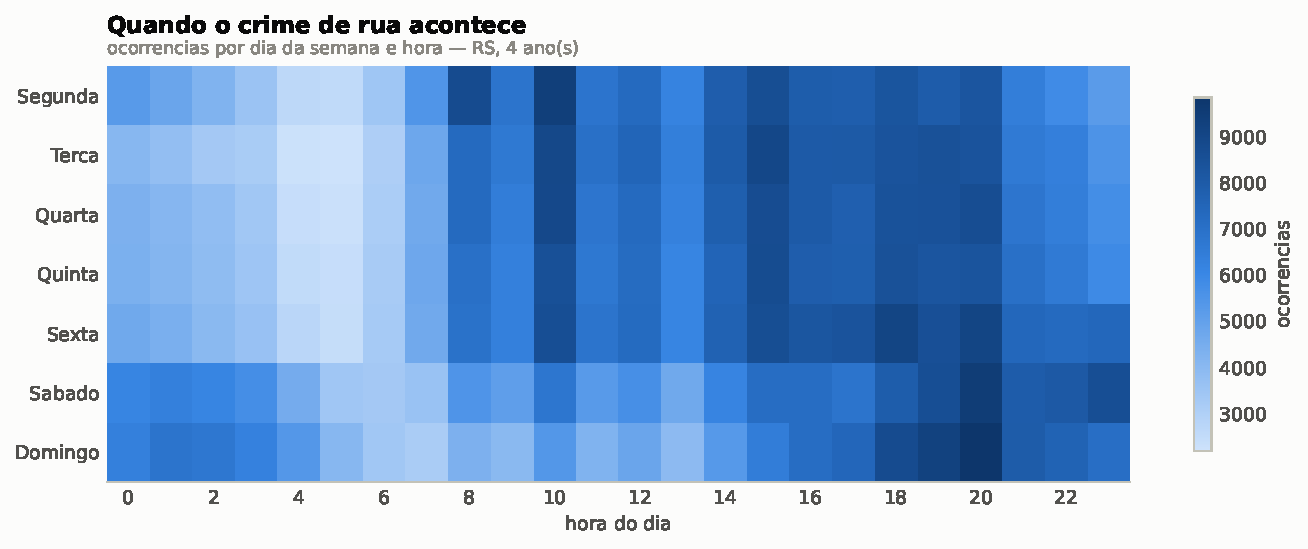
\includegraphics[width=0.92\textwidth]{f1_heatmap_dia_hora.pdf}
    \caption{Ocorrências de crime de rua por dia da semana e hora do dia
    (RS, 2022--2025).}
    \label{fig:heatmap}
\end{figure}

\subsection{Cada crime tem sua hora}
Agregar todos os crimes esconde que cada tipo tem seu horário. A
Figura~\ref{fig:perfil} normaliza a distribuição horária por macrocategoria: o
furto comum concentra-se de dia, ao passo que roubo e lesão sobem à noite. É essa
diferença de perfil que justifica uma escala de policiamento variável por turno,
e não apenas mais efetivo no horário de pico geral.

\begin{figure}[htbp]
    \centering
    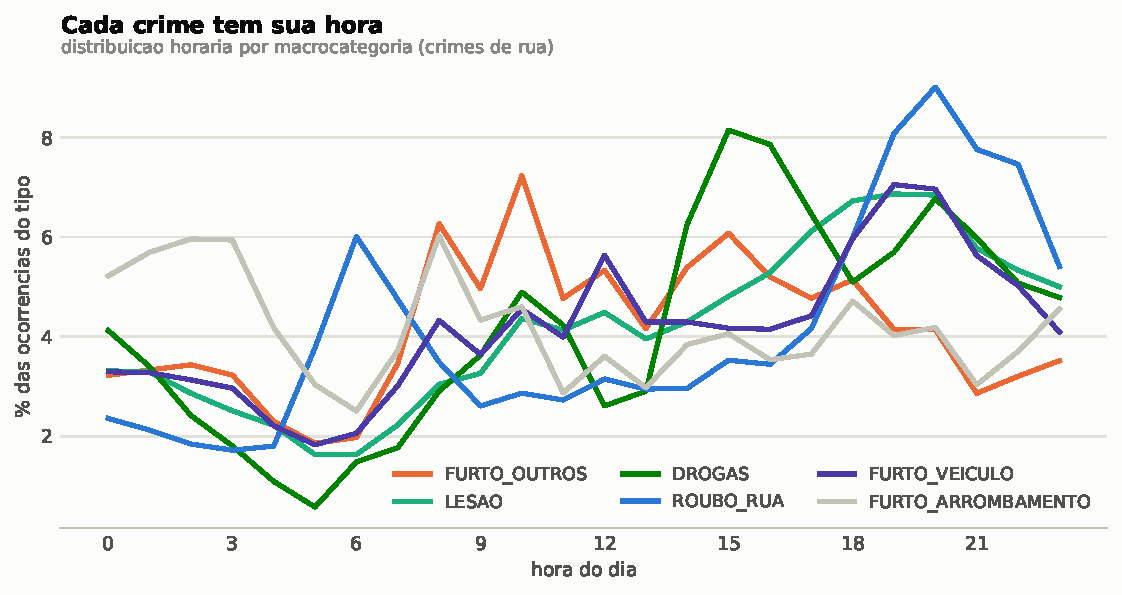
\includegraphics[width=0.9\textwidth]{f2_perfil_horario_por_tipo.pdf}
    \caption{Distribuição horária por macrocategoria (crimes de rua): cada tipo
    tem um horário de pico distinto.}
    \label{fig:perfil}
\end{figure}

\subsection{Onde a taxa é maior}
Convertidas em taxa por habitante, as 15 maiores taxas municipais
(Figura~\ref{fig:municipios}) são dominadas por municípios litorâneos de pequeno
porte --- um artefato que discutimos adiante. Ao restringir a municípios com 50
mil habitantes ou mais (Figura~\ref{fig:grandes}), o quadro se equilibra:
aparecem cidades do interior como Vacaria e Cruz Alta ao lado de Porto Alegre,
mostrando que taxa elevada não é exclusividade do litoral nem da capital.

\begin{figure}[htbp]
    \centering
    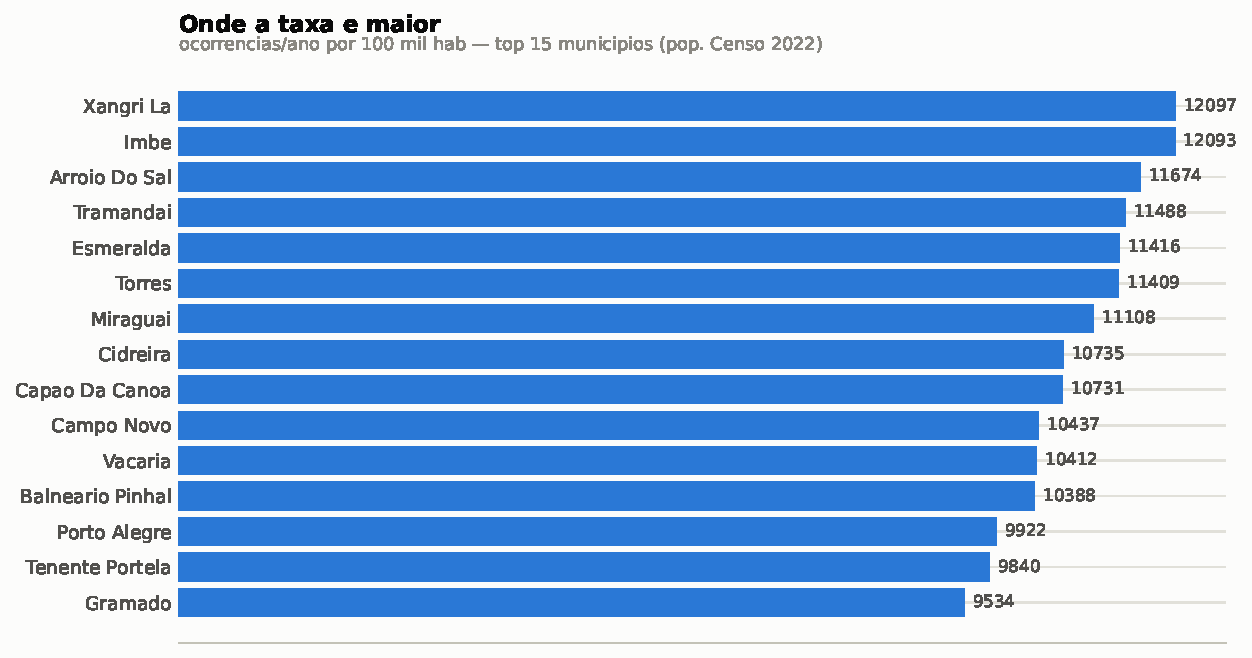
\includegraphics[width=0.82\textwidth]{f3_taxa_municipio.pdf}
    \caption{Taxa média anual por 100 mil habitantes, 15 maiores municípios
    (população: Censo 2022). O topo é dominado por municípios litorâneos.}
    \label{fig:municipios}
\end{figure}

\begin{figure}[htbp]
    \centering
    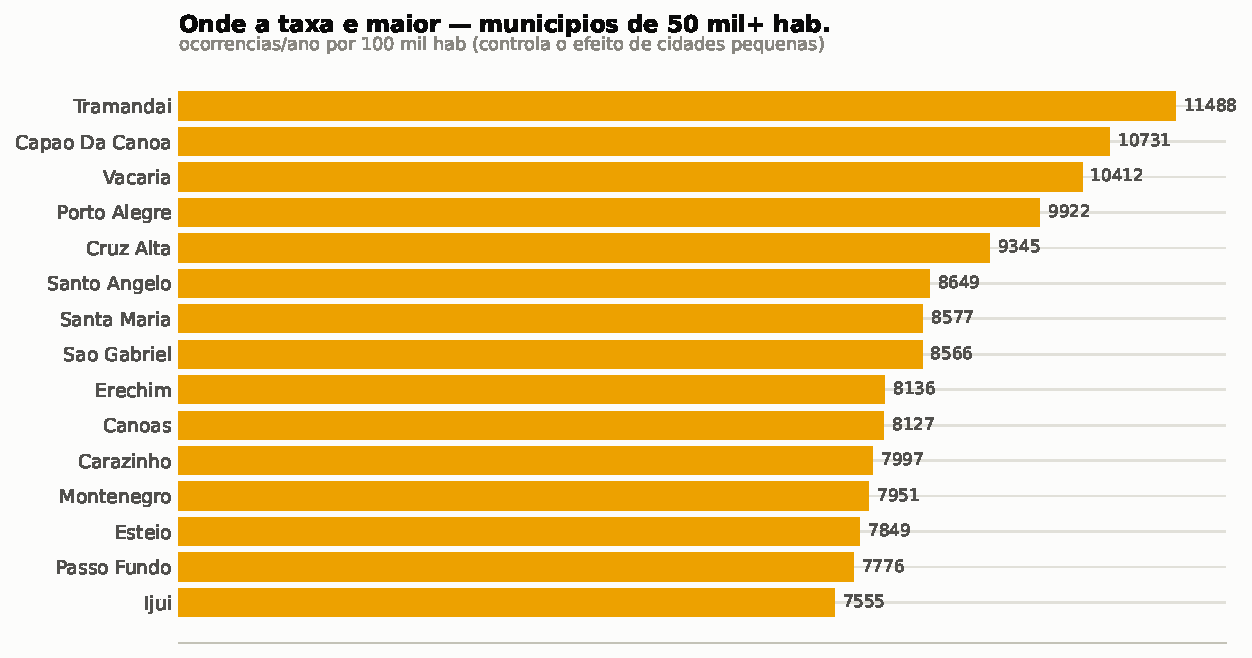
\includegraphics[width=0.82\textwidth]{f3b_taxa_municipio_grandes.pdf}
    \caption{Taxa média anual por 100 mil habitantes entre municípios de 50 mil
    habitantes ou mais, controlando o efeito das cidades pequenas.}
    \label{fig:grandes}
\end{figure}

\subsection{Intensidade por mesorregião}
Agregada por mesorregião e ponderada pela população
(Figura~\ref{fig:mesorregiao}), a taxa varia da região Metropolitana de Porto
Alegre (cerca de 8.000 ocorrências/ano por 100 mil hab.) ao Centro Oriental
(cerca de 5.900), uma diferença próxima de um terço. O teste de Kruskal-Wallis
(Seção~\ref{sec:testes}) confirma que essa diferença entre regiões é
estatisticamente significativa.

\begin{figure}[htbp]
    \centering
    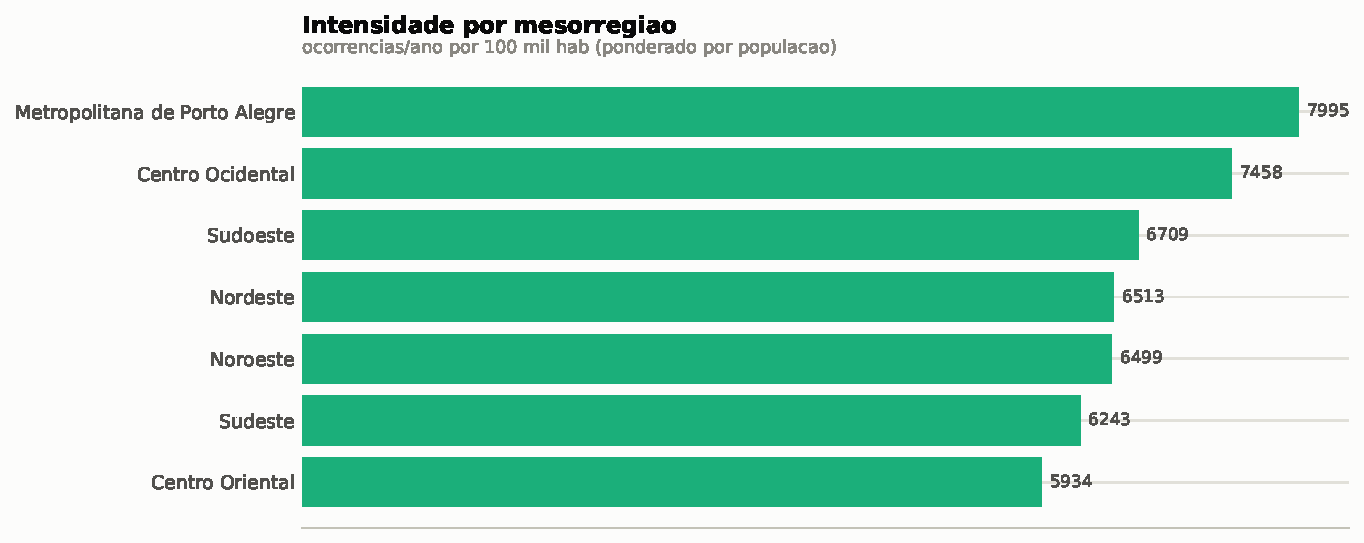
\includegraphics[width=0.82\textwidth]{f4_taxa_mesorregiao.pdf}
    \caption{Taxa média anual por 100 mil habitantes por mesorregião
    (ponderada pela população).}
    \label{fig:mesorregiao}
\end{figure}

\subsection{O pico é a noite em todo o estado}
Cruzando espaço e tempo, a Figura~\ref{fig:turnoregiao} mostra a distribuição dos
crimes de rua por turno \emph{dentro} de cada mesorregião. O resultado simplifica
a decisão: a noite é o turno de maior concentração nas sete regiões, sem exceção.
A diferença regional está na madrugada, que pesa mais no interior (cerca de 21\%
das ocorrências no Sudoeste e no Sudeste) do que na região Metropolitana
(cerca de 15\%).

\begin{figure}[htbp]
    \centering
    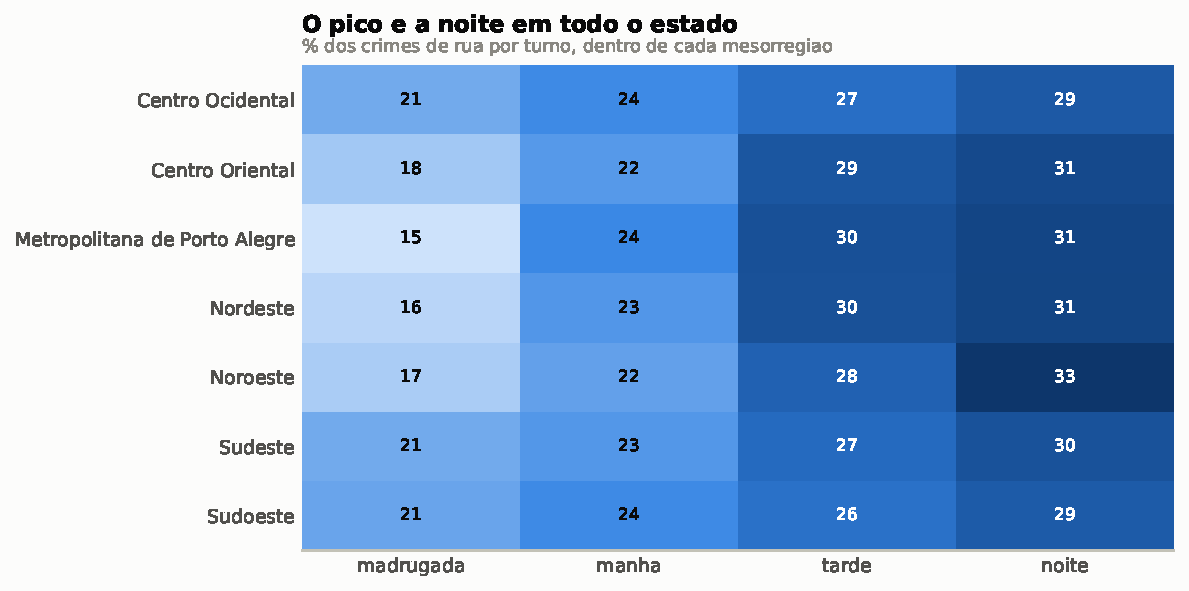
\includegraphics[width=0.75\textwidth]{f7_turno_mesorregiao.pdf}
    \caption{Percentual de crimes de rua por turno dentro de cada mesorregião:
    o pico é a noite em todas.}
    \label{fig:turnoregiao}
\end{figure}

\subsection{Sazonalidade: o efeito do veraneio}
A liderança dos municípios litorâneos na taxa por habitante tem explicação. A
Figura~\ref{fig:sazonalidade} contrasta a distribuição mensal das ocorrências no
litoral e no restante do estado: enquanto o interior é praticamente plano ao
longo do ano, o litoral salta para 12,5\% de suas ocorrências em janeiro (contra
8,6\% no resto), com novo pico em dezembro. O padrão coincide com a temporada de
veraneio, quando a população \emph{presente} é muito maior que a residente do
Censo --- o que infla artificialmente a taxa anual desses municípios.

\begin{figure}[htbp]
    \centering
    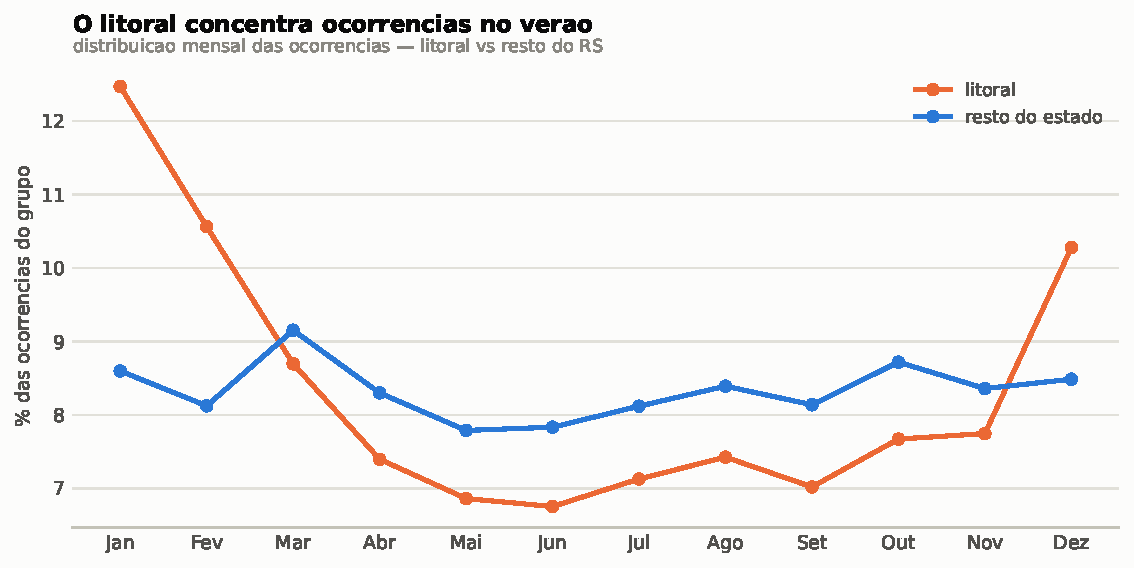
\includegraphics[width=0.9\textwidth]{f6_sazonalidade_litoral.pdf}
    \caption{Distribuição mensal das ocorrências: litoral \emph{versus} restante
    do estado. O litoral concentra ocorrências no verão.}
    \label{fig:sazonalidade}
\end{figure}

\subsection{Testes de hipótese}\label{sec:testes}
O qui-quadrado entre macrocategoria e turno rejeita a independência
($\chi^2 = 40{.}607$, $\mathrm{gl} = 24$, $p \approx 0$): o tipo de ocorrência
\emph{não} é independente do turno. Com 3,1 milhões de registros, porém, a
significância é praticamente garantida; o que importa é a magnitude, e o $V$ de
Cramér de $0{,}11$ indica uma associação real mas modesta --- o turno molda o
\emph{tipo} de crime, sem determinar a sua ocorrência. Os resíduos padronizados
(Figura~\ref{fig:residuos}) revelam o padrão: o furto por arrombamento concentra
na madrugada, o furto comum de manhã e à tarde, e roubo e lesão à noite; as
mesmas células mostram forte \emph{ausência} onde o crime não ocorre (o furto
comum praticamente some à noite).

O qui-quadrado entre macrocategoria e mesorregião também rejeita a independência
($\chi^2 = 50{.}368$, $\mathrm{gl} = 48$, $p \approx 0$; $V = 0{,}09$): o perfil
de crimes varia entre regiões, novamente com efeito modesto. Por fim, o teste de
Kruskal-Wallis sobre a taxa por 100 mil habitantes dos municípios, agrupados por
mesorregião, confirma diferença significativa entre as regiões
($H = 30{,}3$, $p \approx 3{,}4\times10^{-5}$).

\begin{figure}[htbp]
    \centering
    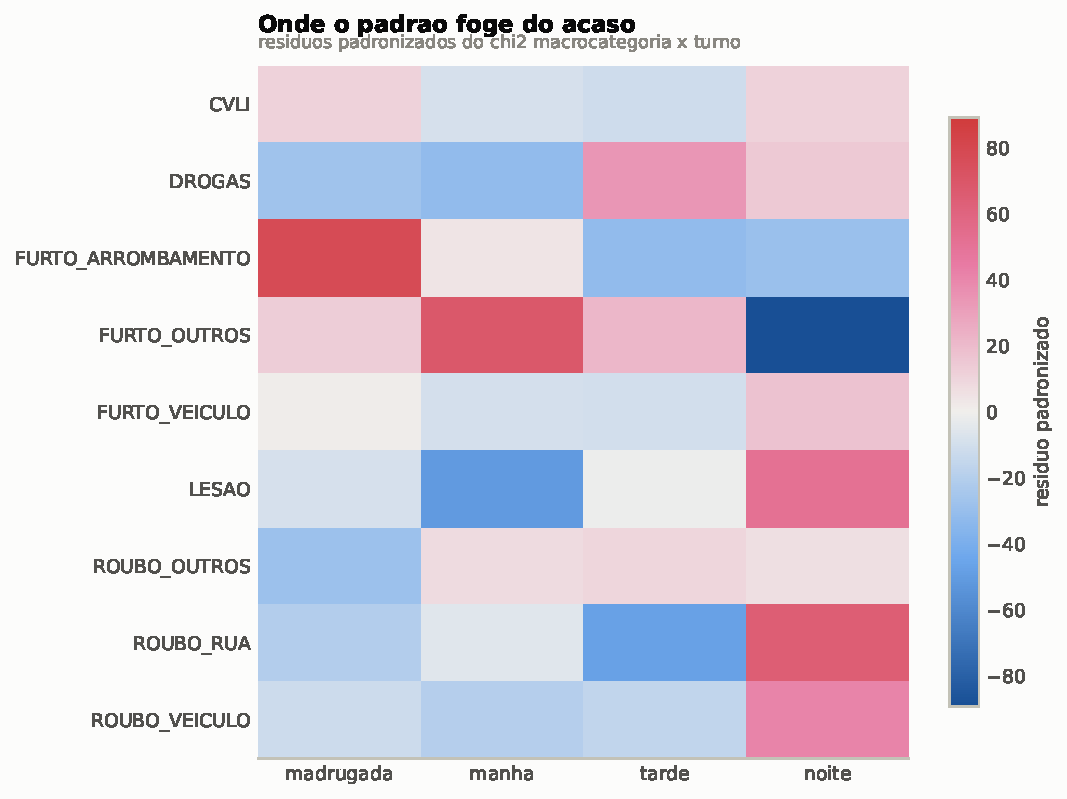
\includegraphics[width=0.7\textwidth]{f5_residuos_chi2.pdf}
    \caption{Resíduos padronizados do $\chi^2$ (macrocategoria $\times$ turno):
    vermelho ocorre mais que o esperado sob independência; azul, menos.}
    \label{fig:residuos}
\end{figure}

% ============================================================================
\section{Limitações}\label{sec:limitacoes}
% ============================================================================
Quatro limitações qualificam as conclusões. Primeiro, o dado mede
\textbf{ocorrência registrada}, não crime real: a subnotificação varia por tipo
de crime e por região, de modo que parte do padrão espacial pode refletir
diferenças na propensão a registrar. Segundo, a \textbf{população de referência}
é a residente do Censo 2022, e não a população presente; como mostra a
Figura~\ref{fig:sazonalidade}, os municípios litorâneos aparecem com taxa inflada
pela população flutuante do verão, e sua taxa anual superestima o risco do
morador fixo. Terceiro, \textbf{municípios pequenos} têm poucos casos e, portanto,
taxas instáveis, com grande variância. Quarto, o \textbf{recorte} é o RS em
2022--2025; as conclusões não se estendem automaticamente a outros estados ou
períodos.

% ============================================================================
\section{Conclusão e recomendação}\label{sec:conclusao}
% ============================================================================
A criminalidade no Rio Grande do Sul não se distribui ao acaso, nem no tempo nem
no espaço. No tempo, o tipo de ocorrência depende do turno --- de forma
significativa, ainda que modesta em magnitude ---, com um padrão nítido:
arrombamento de madrugada, furto de dia, roubo e lesão à noite. No espaço, a taxa
por habitante difere entre as mesorregiões. E o cruzamento das duas dimensões
simplifica a decisão: o pico é a noite em todas as regiões.

\textbf{Portanto, a recomendação} para a SSP-RS é uma escala de policiamento
\emph{uniforme quanto ao pico} --- reforço noturno em todo o estado --- e
\emph{diferenciada quanto à composição}: patrulhamento ostensivo noturno contra
roubo e lesão nos centros urbanos, e vigilância de madrugada contra arrombamento,
com peso maior no interior, onde a madrugada é mais crítica. Na priorização entre
municípios, o critério deve ser a taxa por habitante (Figura~\ref{fig:grandes}), e
não o volume bruto.

\textbf{Com a ressalva de que} o dado é de ocorrência registrada, sujeito a
subnotificação desigual; de que a taxa usa a população residente, o que faz o
litoral parecer de alto risco permanente quando na verdade seu problema é
sazonal --- devendo ser tratado com reforço no verão, e não como prioridade o ano
todo; e de que a associação estatística encontrada, embora real, é de magnitude
modesta, e deve orientar a alocação sem substituir o conhecimento operacional de
cada comando regional.

% ============================================================================
% REFERENCIAS
% ============================================================================
\begin{thebibliography}{9}
\bibitem{sspRS}
Secretaria da Segurança Pública do Rio Grande do Sul.
\textit{Dados abertos --- Ocorrências criminais}.
Disponível em: \url{https://ssp.rs.gov.br}. Acesso em: 16 set. 2026.

\bibitem{ibgeCenso}
Instituto Brasileiro de Geografia e Estatística (IBGE).
\textit{Censo Demográfico 2022 --- População residente por município} (API de
Agregados) e \textit{API de Localidades} (mesorregiões).
Disponível em: \url{https://servicodados.ibge.gov.br}. Acesso em: 16 set. 2026.

\bibitem{scipy}
Virtanen, P. et al. \textit{SciPy 1.0: Fundamental Algorithms for Scientific
Computing in Python}. Nature Methods, v. 17, p. 261--272, 2020.
\end{thebibliography}

\end{document}
